\chapter{Maximum likelihood estimation} \label{mle}
\index{maximum likelihood estimation|ff}
\index{MLE|see{maximum likelihood estimation}}

Maximum likelihood estimators (MLEs) are the bread and butter of
statistics.  Most of the techniques discussed so far are MLE
techniques, except mathematicians over the ages have found ways to hide
that fact from you, by proving that under certain conditions the
maximum must have an easy-to-calculate form. But if there is not a nice,
convenient shortcut, you will have to search for the optimal parameters
yourself. There are optimization routines from a variety of sources,
and Apophenia provides a consistent front-end to many of them via its
\cind{apop\_maximum\_likelihood} function. You give it a function and
some parameters, and it will find the optimum.

\paragraph{The \ind{log likelihood function}}	\label{the score}
By itself, the PDF is the likelihood that a given value occurs (given
the parameters of the PDF); any of the functions listed in Section
\ref{distlist} will do. That distribution, say $P(x|p)\sim$ Bernoulli,
plus a given value for the parameter(s) $p$, will tell us the likelihood
that we would get the data point that we saw. Or, we could reverse this:
given the data $x$, we can use the Bernoulli distribution to calculate the
likelihood that $p$ has any given value.

Say that we have two data points, $x_1$ and $x_2$. Assume further that
they are independently drawn.  The independence assumption allows us
to say the the joint probability is the product of the individual
probabilities; that is, $P(\{x_1,x_2\}|p)=P(x_1|p)\cdot P(x_2|p)$.
The assumption of identical distributions allows us to write this more
neatly, as $$P(\{x_1,x_2\}|p)=\Pi_{i=\{1,2\}}P(x_i|p).$$

Define the Log likelihood as $L=\ln P$, the Score\index{score} as

$$S={\partial \ln P\over \partial \theta}$$ 

and the Information variable\index{information variable} as

\begin{eqnarray}
I&=&-{\partial S \over \partial \theta}			\nonumber\\
&=&-{\partial^2 L \over \partial \theta^2}.		\nonumber
\end{eqnarray}

First, due to all that exponentiation in the distributions
of Section \ref{distlist}, $L$ is often much easier to deal with, yet
is equivalent to the PDF for most of our purposes---notably, if we have
found a maximum for one, the we have found a maximum for the other.

\label{precisionfix}
Further, consider calculating the likelihood function above given
a thousand data points.  Then the probability of observing the data set
we have (fixing $p$ for now) is $\prod_{i=1}^{1000} P(x_i)$.  Since each
$P(x_i)\in (0,1]$, this product is typically on the order of $1\times
10^{-1000}$. This is a delicate number, and details of implementation in
memory could easily break it; this risks what computer scientists call an
{\sl underflow error} (see page \pageref{precisionproblem}). Taking logs, each value of $p_i$ is now a negative
number, e.g., $\ln(0.5)\approx -0.69$ and $\ln(0.1)\approx -2.3$.  But the
product above is now a sum: $$\ln\left[\prod_{i=1}^{1000} P(x_i)\right]
= \sum_{i=1}^{1000} \ln\left(P(x_i)\right).$$ Thus, the log likelihood of our typical
data set is on the order of -1000 instead of $1\times 10^{-1000}$---much
more robust and manageable.\footnote{Zero probability events are still
a problem: they make the original likelihood product zero, and the log
likelihood $-\infty$. The problem is that if a statistical model
specifies a zero-probability event, and that event happens, then the
model is proven false, and the likelihood function shows it. Near-zero
probability events can have a disproportionately large effect on the
parameter estimation, so care must be taken to evaluate whether events with very
small probability should be taken as signs that the model is false,
should be handled as outliers, or should simply be taken as 
measurement error.}

\marginalia{15}{\ind{Exponential families}}{%
	There is a bit of a sleight of hand in asserting that $S \cdot P = {\partial P
\over \partial \theta}$: the derivative of the expectation is
	${d\over d\theta}\int P dy$, while we want $\int {d P\over
	d\theta} dy=\int S \cdot P dy$ [Note how this means $E(S)=0$, by the
	way, since the integral of the PDF is one, and $d1/d\theta=0$].
	If we can't reverse the integral and derivative like this, none
	of this applies. But we can in the case of any exponential
	family. You can look that up, but here, we can rest assured that
	the \ind{Normal}, \ind{Gamma}, \ind{Beta}, \ind{Binomial}, \ind{Poisson}, \&c. are all exponential
	families.} 
The second benefit to using the log likelihood is analytic: since $S \cdot
f = {\partial f \over \partial \theta}$, the derivative of the expectation
in terms of $\theta$ can be rewritten as the expectation of $S$. See box
at left for a few details.

There are some fun tricks you can do with these functions.
The trick most worth mentioning is the
\ind{information equality}, that $E(I)=\var(S)$, which you can prove by
calculating ${\partial E(L)\over \partial \theta}$.

The reader can also verify that 
\begin{align}
\frac{\partial \ln P}{\partial \theta}\cdot \frac{\partial \ln P}{\partial \theta} &= -\frac{\partial^2 \ln P}{\partial \theta^2}.\nonumber\\
\intertext{That is,}
S\cdot S &= -I.\nonumber
\end{align}


\subsection{An example: probit} \index{probit|(}
The probit is a popular model of aleatory behavior. 
Let the utility from vector $\xv$ be 
$U(\xv|\betav) = \beta_0 + \beta_1 x_1 + \beta_2 x_2 + \beta_3 x_3 + \beta_4 x_a + \epsilon$,
where the $\beta$s are all parameters to be estimated from
the data and $\epsilon \sim {\cal N}(0,1)$.
Then a person consumes $\xv$ iff $U(\xv|\betav)>0$. 

An equivalent way to put the model is to say that $U(\xv)$ is
deterministic---drop $\epsilon$ from the above, and let the probability that
the agent consumes be
$$P(\xv|\betav) = \int_{-\infty}^{U\left(\xv|\betav\right)} {\cal N}(0,1)(y) dy,$$
where ${\cal N}(0,1)(y)$ indicates the Normal PDF at $y$ (and so the
integral is the CDF up to $U(\xv|\betav)$).

Reversing this, the probability of $\betav$ given that the agent
consumed is $P(\xv)$, and its probability given that the agent did not
consume is $1-P(\xv)$. Let $\xv^C$ be the set of $\xv$s that led to
consumption and $\xv^N$ be the set that led to nonconsumption. Then the
likelihood of $\betav$ given the data set is 
$$L(\betav|\xv) = \prod_{i} P(\xv^C_i|\betav) \cdot \prod_{i} \left(1-P(\xv^N_i|\betav)\right).$$ 

One row of our data set will consist of a one or zero indicating
consumption or non-consumption, and then (the transpose of) the vector
$\xv$. Then the probit parameters can be estimated using
\cinline{apop\_probit.est\-i\-mate(data, NULL)}.
\index{probit|)}

\section{Why likelihood functions are great} The process of finding a
maximum of the log likelihood function is 
useful for two reasons, with four names: the Cramer-Rao lower bound and
the Neyman-Pearson lemma.

\paragraph{MLEs achieve the Cramer-Rao lower bound} 
        \index{Cramer-Rao Inequality|(}		\label{cr} 
Say we have an unbiased estimator of $\theta$,
$\hat\theta(y_1,\dots,y_n)$. Cramer \& Rao say:
\begin{eqnarray}
\var(\hat\theta)&\geq&(n \var(S))^{-1}		\nonumber\\
		&=&\left(nE\left({\partial^2 L\over \partial
\theta^2}\right)\right)^{-1}			\label{CRLB}
\end{eqnarray}

\comment{
A sketch of the proof: Take my word for it that $E(\hat\theta
\overline S)={1\over n}$. Since $\overline S=0$, that's equivalent to
$\cov(\hat\theta, \overline S)={1\over n}$.  Plug that into Cauchy-Schwarz:
$\var(\hat\theta)\var(\overline S)\geq {1\over n^2}$. Plug
$\var(S)=n\var(\overline S)$ in to that, and the first line of the above
drops out\cite{goldberger}. The second line uses the information
equality from above.

Just remember: the Cramer-Rao lower bound is the inverse of $n$ times
the expectation of the derivative of the derivative of the log of the
likelihood function.
	}

The Cramer-Rao lower bound is
called a `lower bound' because Mr.s Cramer and Rao proved that any
estimator of $\theta$ must have a variance greater than or equal to the
CRLB. Your favorite probability textbook (e.g., \cite{casella:berger})
will also prove that for the MLE, the variance is actually equal to the
CRLB, meaning that we can not get an estimator of $\theta$ that will
have a smaller variance.
        \index{Cramer-Rao Inequality|)}

\subsection{How to evaluate a test}
A test will either reject or accept a hypothesis given data. It can be
fooled two ways: the hypothesis could be true but the test rejects it;
or the hypothesis could be false but the test accepts it anyway. 

\marginaliafixed{16}{Evaluation vocab}{
%\marginalia{Evaluation vocab}{
Here are some vocabulary terms; if you are in a stats class right now,
you will be tested on this:

Likelihood of {\bf Type I errors} $\equiv\alpha$: rejecting the null when it is true.

Likelihood of {\bf Type II errors} $\equiv\beta$: accepting the null when
it is false.

{\bf Power}$\equiv 1-\beta$, or the likelihood of rejecting a false null.\index{power}

{\bf Unbiased}$\equiv (1-\beta)\geq \alpha\ \forall$ values of the parameter.
I.e., you are less likely to accept the null when it is false than when
it is true.\index{unbiased estimator}

{\bf Consistency}$\equiv$ the power $\to 1$ as $n\to \infty$.\index{consistency}
}

There
is a balance to be struck between the two errors: as one rises, the
other falls. But not all estimators are born equal: if a hypothesis has a 50-50 chance of being true, then the coin-flip test, `heads, accept;
tails, reject' gives us a 50\% chance of a Type I error
and a 50\% chance of a Type II error, but there are tests where both
errors are significantly lower than 50\%, and so by any measure we would
call those better tests than the coin-flipping test. 

\paragraph{Keeping Type I and Type II straight} 
\index{Type I error|textbf} \index{Type II error|textbf}

Think of the null hypothesis as on
trial \citep[pp 112--113]{kmenta}.  The rulings a jury may return are
not \airq{guilty} and \airq{innocent}, but \airq{guilty} and \airq{not
guilty}. Most citizens feel that to convict a not-guilty person is a worse
error than freeing a guilty person. So, we list the conviction of the
not-guilty---rejecting $H_0$ when it should not have been rejected---as
Type I, and the secondary error of acquitting the guilty---failing to
reject a false $H_0$---as Type II.


\subsection{The Neyman-Pearson lemma} \index{Neyman-Pearson lemma} 
The other reason that we ignore Type II errors is that Neyman and Pearson
told us we could.  They showed that a likelihood ratio test will have
the minimum possible Type II error of any test with the $\alpha$ that
we selected. After establishing this fact, we just ignore Type II errors.

\paragraph{Likelihood ratios} \index{likelihood ratio|ff}

Say the cost to a Type I error is $C_I$ and the cost to a Type II error
is $C_{II}$.  Then it is sensible to reject $H_0$ iff the expected cost is less
than the likely cost of not rejecting. That is, reject $H_0$ iff $C_I
P(H_0|\xv)<C_{II} P(H_1|\xv)$.

We need to note two things from here. First, the difference between a
`probability', which is the probability of an event given data; and a
`likelihood', which is the probability that we'd have the data we have
given some event. This is primarily just vocabulary, because in many
senses, the two are identical.\footnote{One could write $P(A|B)$ as a symmetric two-variable function:
$P(A,B)$, with the understanding that $\int_{\forall A} P(a,B)da = 1,
\forall B$.} 

Second, ?`remember the definition of a \ind{conditional probability}? It's based on the
statement $P(A\cap B)=P(A|B)P(B)$, and symmetrically, $P(A\cap B)=P(B|A)P(A)$.  Equating
the two and shunting over $P(B)$ gives us \ind{Bayes's rule}: $$P(A|B)={P(B|A) P(A)\over P(B)}$$
Applying Bayes's rule to the rejection test is easy: set $A=H_0$, $B=\xv$,
$P(A|B)=P(H_0|\xv)$, and $P(B|A)=L(\xv|H_0)$. Then:
\begin{align}
C_I P(H_0|\xv)&<&C_{II} P(H_1|\xv)\label{firstnp}\\
\nonumber\\
C_I {L(\xv|H_0)P(H_0)\over P(\xv)}&<& C_{II} {L(\xv|H_1)P(H_1)\over P(\xv)}\label{secondnp}\\
\nonumber\\
c&<& {L(\xv|H_1)\over L(\xv|H_0)}\label{thirdnp}
\end{align}

Inequality \ref{firstnp} is the rejection rule from above; Inequality
\ref{secondnp} uses Bayes's rule to insert the likelihood functions;
Inequality \ref{thirdnp} just does some cross-division, canceling out the
$P(\xv)$s, and defining $c\equiv C_IP(H_1)/C_{II}P(H_0)$, i.e., everything
that doesn't depend on $\xv$. If you tell me the shape of the distribution
and some number $\alpha\in(0,1)$, then I can give you a value of $c$
such that Inequality \ref{thirdnp} is true with probability
$\alpha$. The test will then be: fail to reject $H_0$ iff Inequality
\ref{thirdnp} is true.

Neyman and Pearson\index{Neyman-Pearson lemma} proved\footnote{See
e.g. \citet[189--191]{amemiya:ez}.}
that this test is the `best' in the sense that for a
fixed Type I error (fixed at $\alpha$), the probability of a Type II
error is minimized. So we can design any test we like by just fixing $\alpha$
at a value with which we are comfortable (custom says to use
90, 95 or 99\%), calculate a few likelihood functions, and we are assured
that we did the best we could regarding Type II errors. You will see that
many of the tests which follow will be of the likelihood ratio form,
and so Type II errors pretty much never get mentioned, since they're
considered taken care of.

\summary{
\item For any sufficiently well-specified model, you can find the
probability that a given data set was produced via the model.
\item If the data set consists of independent and identically distributed elements,
then the likelihood is a product with one term for each data point. 
For both computational and analytic reasons, the log likelihood is
easier to work with; the product then becomes a sum.
\item The parameters that maximize the likelihood function (or 
identically, maximize the log likelihood) will have the minimum variance
among all unbiased estimators. The variance is a known quantity, given
by the Cramer-Rao lower bound, Equation \ref{CRLB}.
\item Type I and Type II errors are complementary: as one goes up,
the other generally goes down. However, given a Type I error level,
different tests will have different Type II error levels.
The Neyman-Pearson lemma guarantees that a likelihood ratio test has the
minimum probability of Type II error for a fixed Type I error level.

}

\section{Description: Maximum likelihood estimators} 
Apophenia provides a single function to find the optimum of a likelihood
function, \cind{apop\_maximum\_like\-li\-hood}---but what a function it is. It
provides a standardized interface to several types of optimization
routines that take very different approaches toward finding optima. You
will have to provide a log likelihood function, but if you are unable to
provide the derivatives, the maximization routines will find them for
you. Since the Cramer-Rao lower bound tells us the variance of a
most-likely parameter, \cinline{apop\_maximum\_likelihood} will return an
\cind{apop\_estimate} with the variances and other useful information.


\subsection{Finding optima} Here is the problem: you want to find the
maximum of $f(\xv)$, but you are only allowed to evaluate the function
and its derivative at a limited number of points. At the extreme,
$f(\xv)$ could be a complex simulation that takes in a few parameters
and runs for an hour before spitting out a value, so you only have time
to evaluate a few dozen points.

This is a classic problem in mathematics and computer science that
continues to be the subject of active research. There is a wide range of
methods available, and which works best for your model depends on its
characteristics. Here are the methods
that are currently supported by Apophenia. The numbers (000, 100, \&c.)
will be used below.

\paragraph{000: The \ind{Nelder-Mead simplex algorithm}} Draws a polygon and
then shifts the corner of the polygon with the smallest function value.
This doesn't require derivatives at all.

\paragraph{100: \ind{Fletcher-Reeves Conjugate gradient algorithm}} This is the
default. Basically, we take the derivative in all directions and find
the linear combination of these directions that indicates the fastest
climb. Clearly, this depends on knowing derivatives; see below.

\paragraph{200: \ind{Broyden-Fletcher-Goldfarb-Shanno Conjugate gradient
al\-go\-ri\-thm}}  Another conjugate gradient method, that calculates the
direction using a \vocab{quasi-Newton algorithm}. Newton algorithms
in many dimensions require first and second derivatives (the Jacobian
and the Hessian), but with a likelihood function of a million terms,
calculating a set of derivatives can be expensive, so the BFGS method
incrementally updates the Hessian using the differential of the function
values calculated.
\index{BFGS algorithm|see{Broyden-Fletcher-Goldfarb-Shanno Conjugate gradient algorithm}} 

\paragraph{300: \ind{Polak-Ribiere Conjugate gradient algorithm}} Yet another
conjugate gradient method, that generally works better for functions
that digress significantly from quadratic.  See \citet[thorough, mathematician audience]{avriel:nonlinear}
or \citet[practical, modeling audience]{practical:optimization}  for definitions of all of these methods.

\paragraph{500: \ind{Simulated annealing}} A controlled random walk.
As with the other methods, the system tries a new point, and if it
is better, switches. Initially, the system is allowed to make large
jumps, and then with each iteration, the jumps get smaller, eventually
converging. Also, there is some decreasing probability that if the new
point is {\em less} likely, it will still be chosen. One reason for
allowing jumps to less likely parameters is for
situations where there may be multiple local optima. Early
in the random walk, the system can readily jump from one to another;
later it will fine-tune its way toward the optimum. Other motivations
for the transition rules will be elucidated in the chapter on Monte
Carlo methods.

The number of points tested is basically not dependent on the function:
if you give it a 4,000 step program, that is basically how many steps
it will take.  If you know your model is globally convex (as are most
standard probability functions), then this method is overkill; if your
model is a complex interaction, simulated annealing may be your only
bet. It does not use derivatives, so if the derivatives do not exist or
are ill-behaved, this is appropriate, but if they are available either
analytically or via computation, then the methods that use derivative
information will converge faster.

\paragraph{Which to choose?}
As a practical matter, your best bet is to either just go with the default
(Fletcher-Reeves) or try them all using a tournament as described below.

The conjugate gradient algorithms are based on a Taylor expansion cut
off at the second term. If your function is quadratic, then they will
converge in one step.  
If approximating your function with a quadratic is not terrible, then
use the default (FR). If the derivatives are smooth but sometimes take sharp
turns, the other conjugate gradient methods (BFGS or PR) may work
better. If you expect the derivatives to be discontinuous or otherwise
perverse  but the functional
values to generally move in one direction, then 
try the derivative-free simplex algorithm. Finally, if the functional
values jump around, so there is a good risk of multiple
optima in odd places, then try simulated annealing.

\paragraph{Global v local optima}
None of the methods guarantee that the optimum found is the global
optimum, since there is no way for a computer to have global knowledge
of a function $f(x)$ for all $x \in (-\infty, \infty)$. One option is
to restart the search from a variety of starting points, in the hope
that if there are multiple peaks, then different starting points will
rise to different peaks.

The simulated annealing algorithm is designed to deal well with multiple
peaks: as the number of steps in the simulated annealing algorithm $\to
\infty$, the algorithm can be shown to converge to the global optimum
with probability one. However, calculating an infinite number of steps
tends to take an unreasonable amount of time, so you will need to select
a time-to-confidence trade-off appropriate to your situation.


\subsection{\ci{apop\_estimation\_params} for ML estimation}
As in the Probit example, Apophenia's model estimation routines can run
with default values by sending in \cinline{NULL} as the second
argument. However, if you know that the model estimates its parameters
via MLE, then you may be able to improve the estimation routine by
specifying the method and scale of the ML search.

Specifying these parameters simply requires 
filling out a form describing your preferences and then calling the model's \cinline{estimate} method.
The form in question is a \cind{apop\_estimation\_params} structure, that
describes the method, the starting point, the step size, and the
tolerance.
For example:
\cindex{apop\_estimation\_params\_alloc}
\begin{lstlisting}
apop_estimation_params *ep  = apop_estimation_params_alloc());
double  starting_point[2]   = {1,1};
ep->method      = 000;
ep->step_size   = 1e-1;
ep->tolerance   = 1e-5;
ep->verbose     = 1;
ep->starting_pt = starting_point;
apop_gamma.estimate(my_data, ep)
\end{lstlisting}

Here are the parts to the  \cind{apop\_estimation\_params}
structure you need to set. 

\paragraph{The method} The method to use is the sum of the method number
listed above plus the gradient-calculation method.\footnote{There are also two more methods that just aren't hooked in yet. If you
are comfortable exploring the internals of Apophenia, have a look at
the \cinline{wn/wnbridge.c} file. More methods will be forthcoming.}

\index{gradients}
If analytic gradients are available, then those are probably preferable,
but Apophenia will automatically calculate numerical gradients
as necessary.  Since the variance of an MLE is the Cramer-Rao lower
bound (Equation \ref{CRLB}), we will use the gradients to calculate
the variance, so even when using a derivative-free simplex algorithm,
the variance will still be using gradients, somehow derived.

Just in case the analytic gradients don't work out for you, there is a
means of just using the numeric gradients. This is primarily useful for debugging:

\begin{itemize}
\item 0: If (and only if) no gradient is available, use numerical approximations.  (default)
\item 1: Use numerical approximations even if an explicit dlog likelihood is given. 
\end{itemize}

The actual number to input is the sum of the method type above plus the
gradient handling method. Thus the default is equal to 100, for example, and the
Nelder-Mead simplex algorithm forcing numerical derivatives would be
001.\footnote{Yes, 000 reduces to 0 and 001 reduces to 1. The internals
don't care, so use whichever form makes the most sense to you as a human.}


\paragraph{The step size} This is the initial distance that the
algorithm will use to start searching for points. Basically arbitrary
because all of these algorithms are adaptive, meaning that they will
change the step size as they see fit.

\paragraph{Tolerance} The algorithm will stop when it feels
that the calculated log likelihood is changing by less than this amount,
indicating that the search is at a local maximum and the first derivative of
the log likelihood function is nearing zero.

\paragraph{Verbose} Should the search output the points it is evaluating?
This is useful for long evaluations to reassure you that nothing is
broken; for example, some of the GSL's searches can get trapped in two-step loops.
It is probably a good idea to run your search verbosely at least once.
Also, see \cinline{apop\_opts.mle\_trace\_path} below.

\paragraph{Starting point} An array of doubles indicating where you want
your search to begin. Being an array, you can use a form like the above
to initialize it (but if you are using automatic allocation like this, then it will be destroyed when you leave the
function that it was initialized in---remember this if you want to
access the starting point in the \cind{apop\_estimate} that the MLE outputs).


\subsection{Restarting} \cindex{apop\_estimate}
\label{restart} One trick for getting a better estimate is is to solve
for an MLE using a coarse scale and then restarting the procedure at
the point where the first MLE found its solution using a finer scale.
To do this, use \cind{apop\_estimate\_restart}.

The function takes three arguments: a prior estimate that you have
already calculated, a method, and a scaling factor. 

First, the function copies off the \cinline{apop\_estimation\_params}
from the \cinline{apop\_estimate} sent in, and then makes a series of
modifications.  If the new method sent in is -1, then the new MLE will
use the same method as before; otherwise specify one of the methods
listed above. The step size and the tolerance are both multiplied by the
scaling factor sent in (so if this is 1, no change is made). If the
estimated parameters for the original estimate is finite and bounded, then 
the starting point in the new \cinline{apop\_estimation\_params}
structure is set to the estimated value; if some element of the
estimated parameters are infinity or NaN, then the original starting
point is reused.

Then, the ML estimation is run again, and we now have two estimates: the
original and the new one. If the new one has not-finite or NaN values,
then it is thrown out and the original returned. If the new estimate 
has a higher log likelihood, then it is returned, and the old estimate
is deleted.  The less likely estimate (which may be the one you sent in) is freed. That is,
there is no memory leak when you run a tournament like:
\begin{lstlisting}
est = apop_estimate_restart(est, 200, 1);
est = apop_estimate_restart(est, 100, 1e-2);
est = apop_estimate_restart(est, -1, 1e-2);
\end{lstlisting}
The estimate can only get better every time you run
\cind{apop\_estimate\_restart}, so the only cost to running a lengthy
tournament is your time waiting for the estimates to converge.

As above, a search produces only a local maximum. You can increase the
confidence that you have found a global maximum by restarting the search
at a different starting point. 
\begin{lstlisting}
double new_starting_pt[]    = {-1,-1};
est->starting_pt = new_starting_pt;
est = apop_estimate_restart(est, -1, 1);
\end{lstlisting}

\subsection{Graphing the path} All of the methods above consist of
trying a series of candidate points. 
If \index{apop\_opts!mle\_trace\_path@\cinline{mle\_trace\_path}}\cinline{apop\_opts.mle\_trace\_path}
has a name of positive
length, then every time the MLE evaluates the function, then the value
will be output to a table in the database with the given name. You can
then plot this table to get an idea of the path the estimation routine
used to arrive at its MLE.

First, set this variable and run the MLE. The begin/commit wrapper
speeds things up a touch, but this will still be slower than without
taking notes:
\begin{lstlisting}
    strcpy(apop_opts.mle_trace_path, "pathtable");
    apop_query("begin;");
    e   = apop_zipf.estimate(...);
    apop_query("commit;");
\end{lstlisting}
Plotting data is covered fully in Chapter \ref{gnuplot}, but for now,
the function below shows how one would plot the trace.  Notice that
you will want \cinline{splot} for 3-d variables and \cinline{plot} for
2-d. The change in width and pointsize is to remind the eye that the
lines connecting the points only indicate the path the maximizer went
along, not actual values of the function. Figure \ref{searchfig} shows a
sample search path.\index{plotting}

\begin{lstlisting}
static void plotme(char *outfile){
FILE            *f;
apop_data       *traced_path;
    f       = fopen(outfile, "w");  //overwrites. Use "a" to append.
    fprintf(f, "splot '-' with linespoints linewidth 0.5 pointsize 2\n");
    fclose(f);
    traced_path = apop_query_to_data("select * from %s"
            , apop_opts.mle_trace_path);
    apop_data_print(traced_path, "\t", outfile);
}
\end{lstlisting}

Finally, call \ind{Gnuplot} from your command line:
\begin{lstlisting}
gnuplot -persist < plotme
 (or)
gnuplot plotme -
\end{lstlisting}

\begin{figure*}
%\scalebox{0.4}{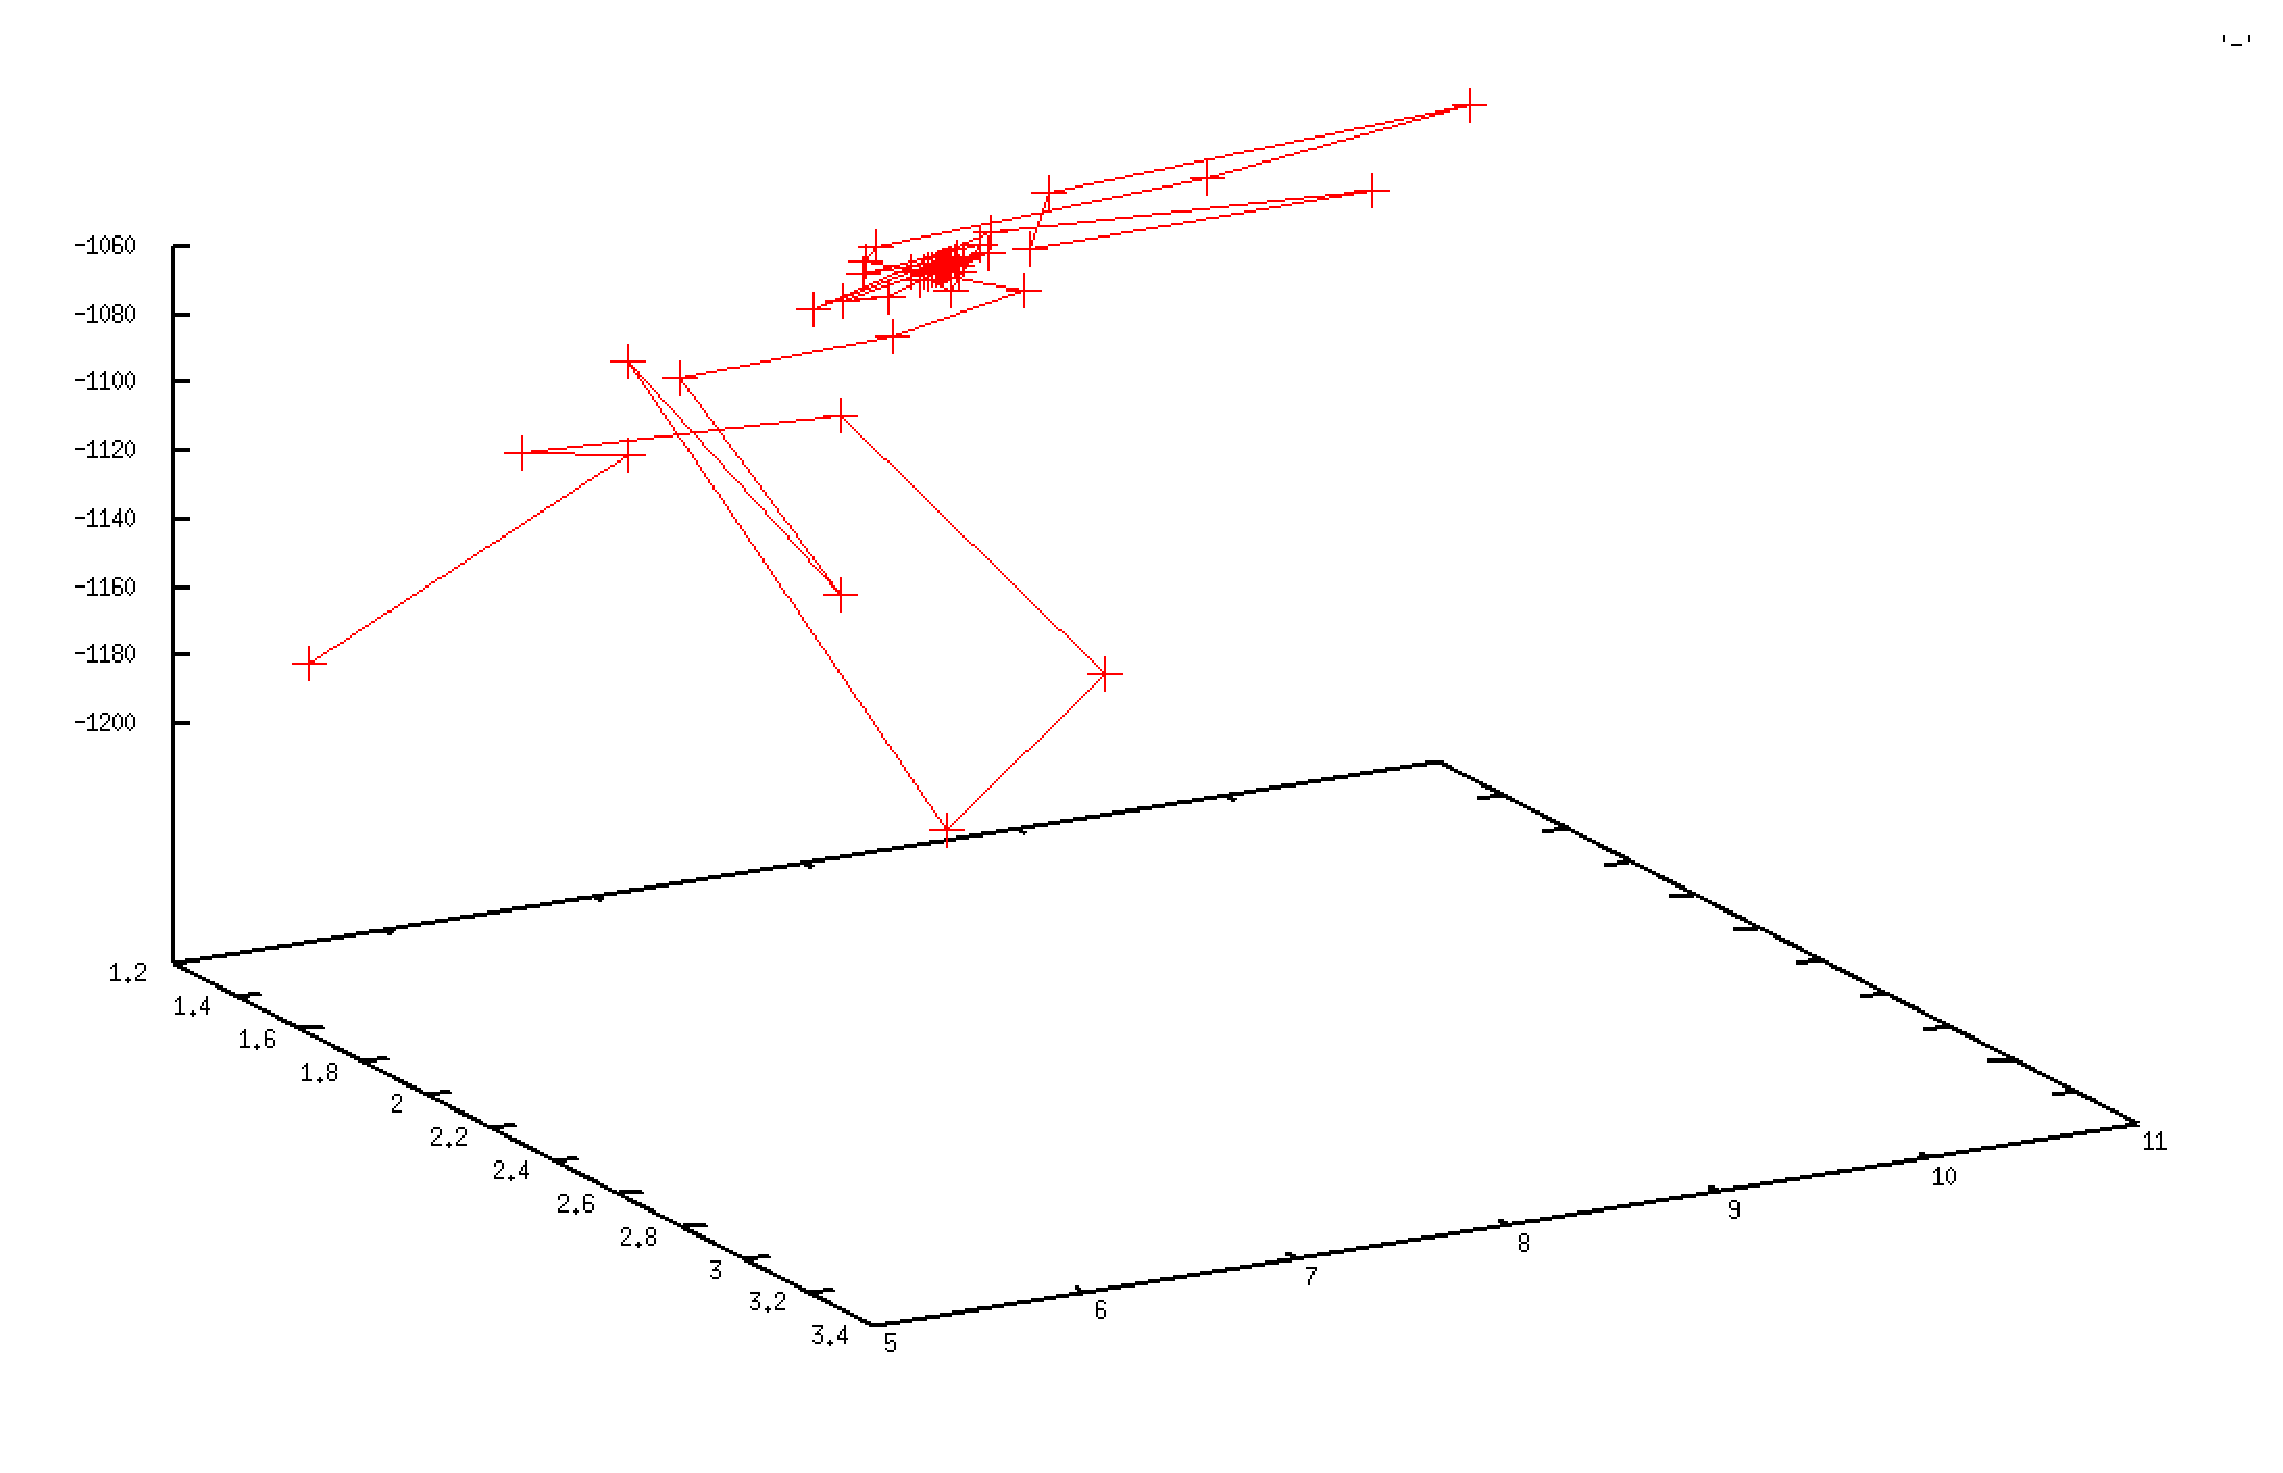
\includegraphics{search}}
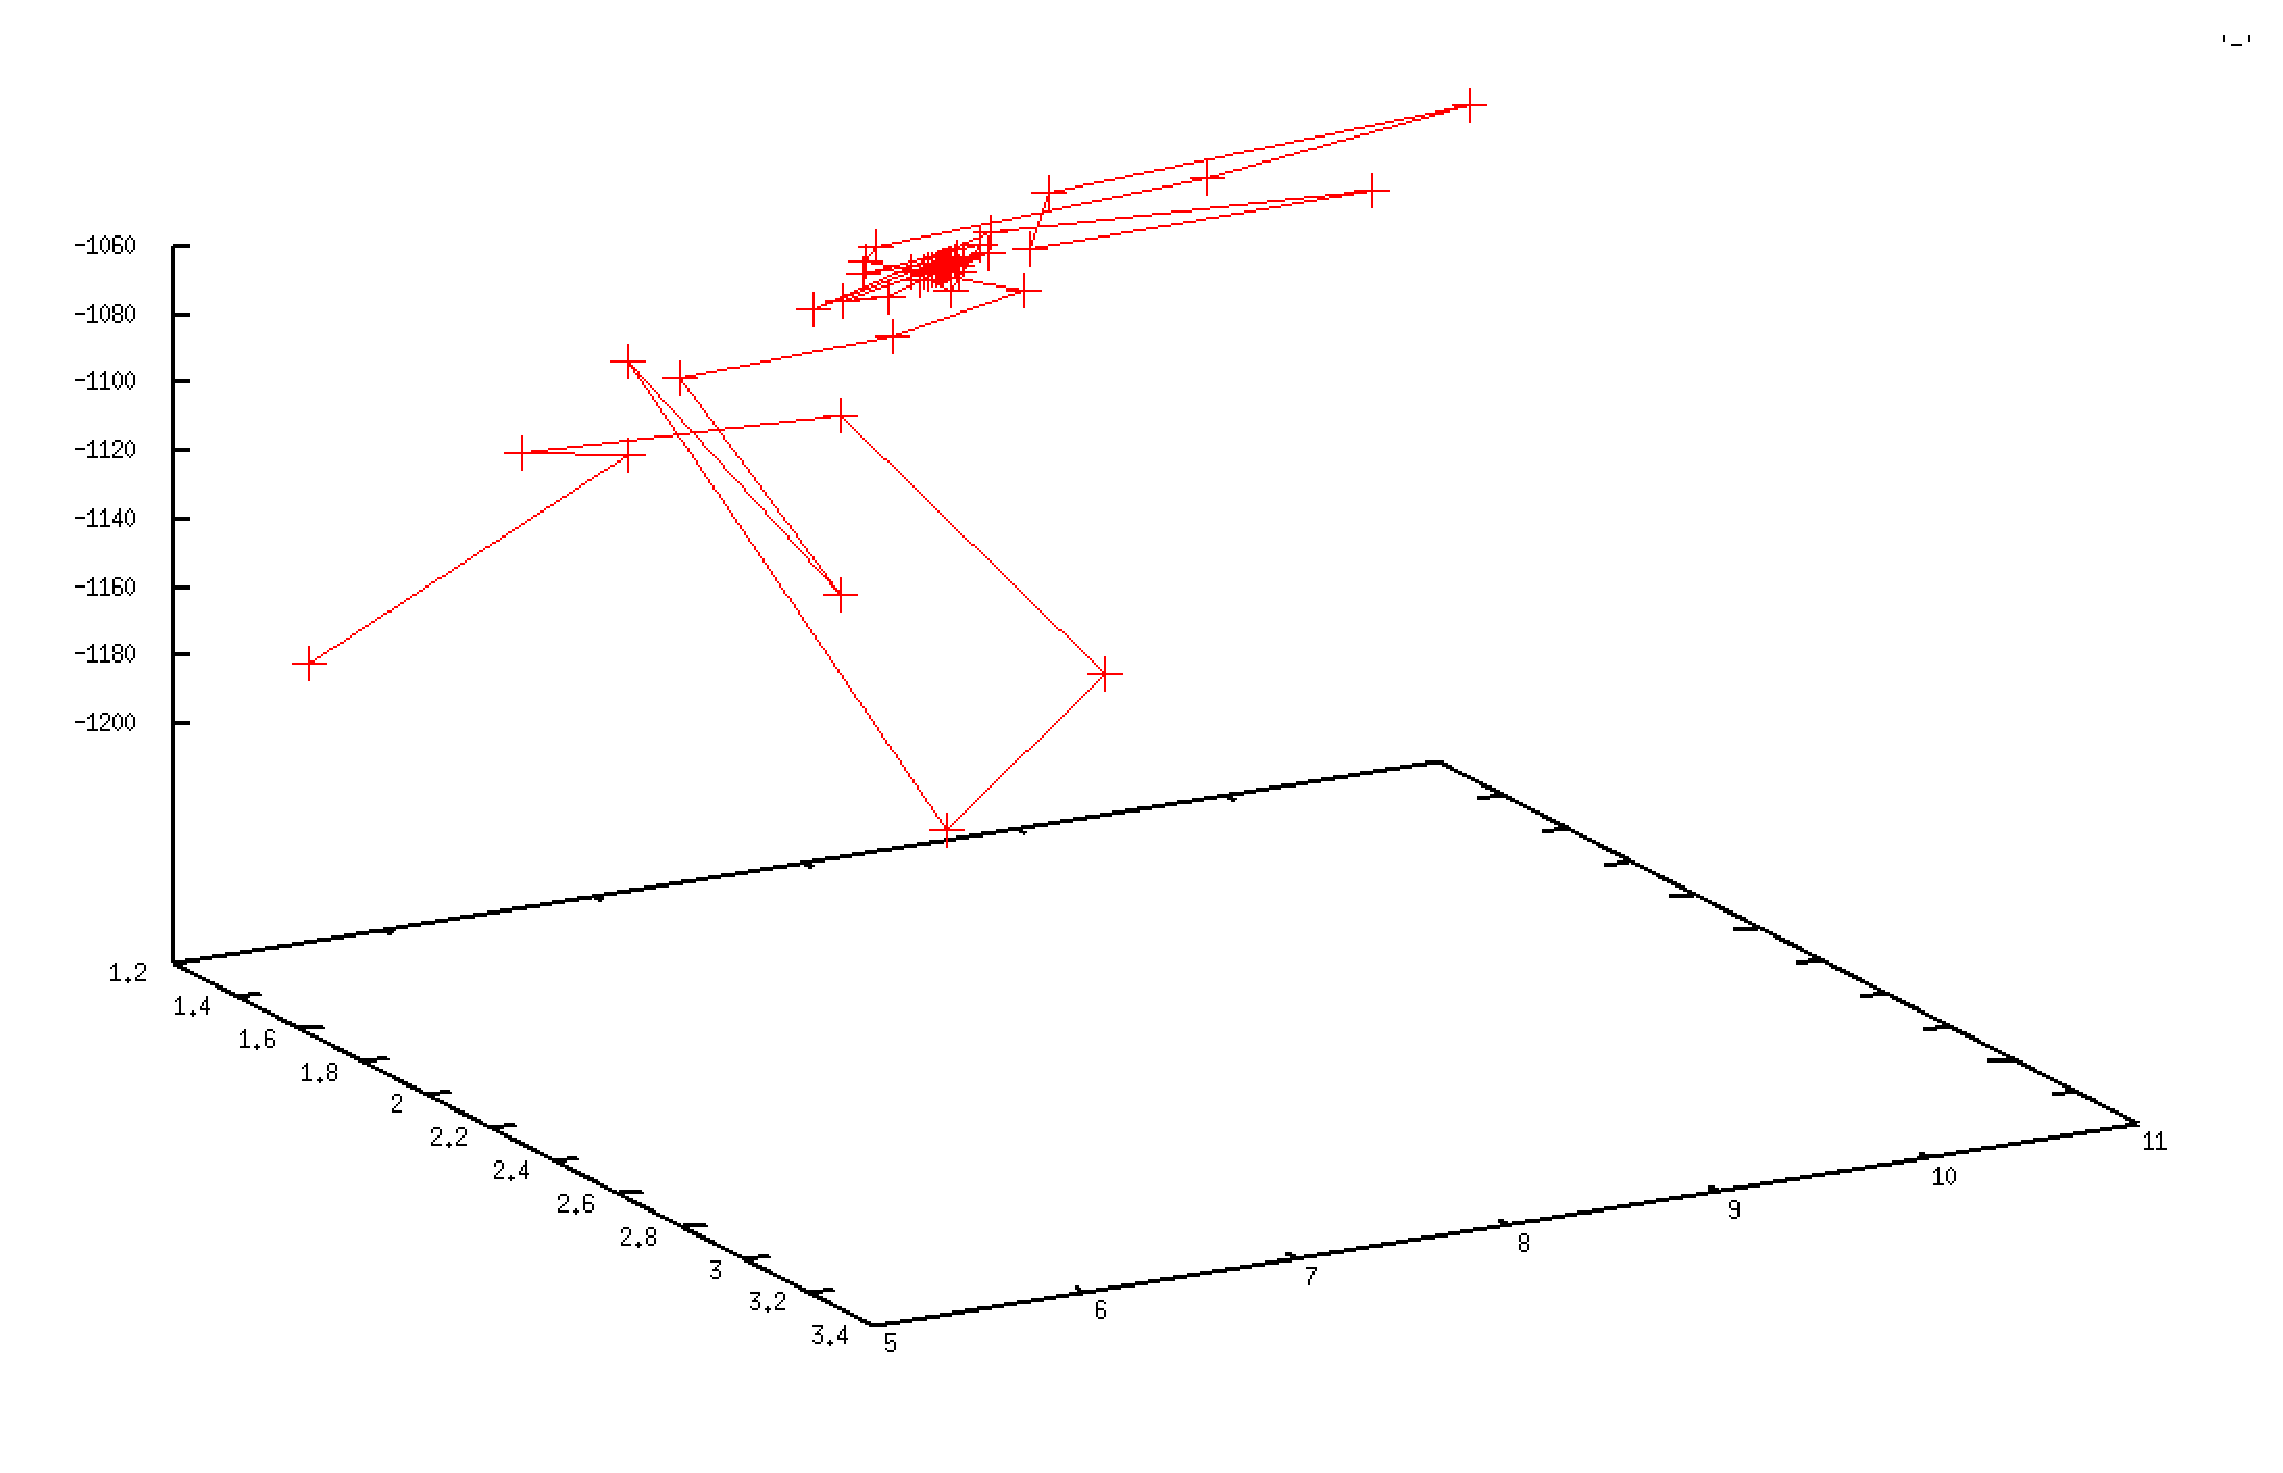
\includegraphics[width=\textwidth*\real{1.1}]{search}
\caption{A search for an optimum using a conjugate gradient method.}
\label{searchfig}
\end{figure*}

\summary{
\item Given an appropriate \ci{apop\_data} set and \ci{apop\_model}, the 
\ci{apop\_maximum\_likelihood} function will apply any of a number of
maximum-searching techniques to find the optimal parameters.
\item You can try various methods in sequence using
\ci{apop\_estimate\_restart}. You can also use the restarting technique
to do a coarse search for the neighborhood of an optimum, and then a
fine search for a better estimate.
\item No computational method can guarantee a global optimum, since the
computer can only gather local information about the function.
Restarting the search in different locations may help to establish a
unique optimum or find multiple optima.
}

\section{Hypothesis testing: Likelihood ratio tests} \index{likelihood
ratio test}\index{Neyman-Pearson lemma}
As intimated by the Neyman-Pear\-son lemma, the ratio of two
likelihoods is a good way to test a hypothesis. 

Typically, the likelihood ratio test involves the ratio of an
unrestricted and a restricted model. Let $L$ be the (not-log, plain)
likelihood of the overall model, and $L_0$ be the likelihood of a
model with $K$ restrictions, such as $K$ parameters fixed as zero. Then
$$-2\ln\frac{L_0}{L} = -2[\ln L_0 - \ln L] \sim \chi^2_K.$$

If you have run a maximum likelihood estimate of two models, then you
already have all you need to do a likelihood ratio test. 
If you are using a linear model such as OLS, you can still do a
likelihood ratio test, because OLS is an MLE based on a set of specific
assumptions.

This section forthcoming, along with a bit on nested/non-nested models.

\section{Writing your own} \label{writeyourown}
The design of the \cinline{apop\_model} hopes to make it as easy as
possible for you to write new models. For the most
part, all you need to do is write a log likelihood function, and
\cind{apop\_maximum\_likelihood} does the rest.  

To save you typing in all this, by the way, buried in the Apophenia
source code, in the \binline{model/} directory, is a file named
\binline{apop\_model\_template.c}.  
You can do a global search-and-replace of MODELNAME to insert the name
of the model you are writing (e.g., in vi, \binline{:\%s/MODELNAME/probit/g})
and then rewrite the functions as per the guidelines here. The template
is not entirely blank: it includes a bit of code that is common to many
models, that you may keep or delete as you prefer.

The steps:

\begin{itemize}
\item Write a likelihood function. Its header will look like this:
\begin{lstlisting}
static double apop_new_log_likelihood(const gsl_vector *beta, apop_data *d)
\end{lstlisting}
where \cinline{beta} will be the parameters to be maximized, and \cinline{d} is the fixed parameters---the data. 
This function will return the value of the log likelihood function at the given parameters.

\item Is this a constrained optimization? See Section
\ref{constraintwriting} on how to write a constraint function.

\item Write the \cinline{estimate} method, so users can call 
\cinline{apop\_new\_like\-li\-hood.\-est\-i\-mate(...)}. For an MLE, this will be one line,
as follows:
\begin{lstlisting}
static apop_estimate * new_estimate(apop_data * data, void *parameters){
    return apop_maximum_likelihood(data, apop_new_log_likelihood, parameters);
}
\end{lstlisting}
By using the \cind{static} keyword, the function name will only be
known to this file, so you can name it what you wish.  But since you
will be putting a pointer to the function into an object below, you
can use the above-mentioned 
\cinline{apop\_new\_like\-li\-hood.\-est\-i\-mate(...)}
form to call this function. 


\item Write the object, a process which will consist of filling out
another form. 
\begin{lstlisting}
apop_model apop_new_model = {"The Me distribution", 
            number_of_parameters, 
            new_estimate,
            new_log_likelihood, 
            NULL,   //place dlog likelihood here.
            NULL,   //place constraint fn here.
            NULL    //place RNG here.
            };
\end{lstlisting}
If there are constraints, then replace the appropriate \cinline{NULL} with the right constraint function; see below.
\cinline{number\_of\_parameters} is probably a positive integer like \cinline{2}, but
it is often (the number of columns in your data set -1), in which case,
set \cinline{number\_of\_parameters} to \cinline{-1}.

\item Write your header file so you can include the model in other
modules. Here is the complete header you will need:
\begin{lstlisting}
apop_model apop_new_model;
\end{lstlisting}
Since the \cinline{apop\_model} structure is defined when you \cinline{\#include
$<$apo\-phe\-nia/head\-ers.h$>$}, the compiler already knows all the necessary
details of your model; all you need to do from there is declare that
your model exists.


\item Test. Debug. Retest.

\item Optional: write a gradient for the log likelihood function. This
involves calculating a derivative by hand, which is typically an easy
problem in high-school calculus. The function's header will look like: 
\begin{lstlisting}
void apop_new_dlog_likelihood(const gsl_vector *beta, apop_data *d, gsl_vector *gradient)
\end{lstlisting}
where \cinline{beta} and \cinline{d} are fixed as above, and \cinline{gradient} is a \cinline{gsl\_vector} with dimension matching \cinline{beta}. 
At the end of this function, you will have to assign the appropriate derivative to every element of the gradient vector:
\begin{lstlisting}
gsl_vector_set(gradient, 0, d_a);
gsl_vector_set(gradient, 1, d_b);
\end{lstlisting}
Now add the resulting dlog likelihood function to your object, by
replacing the \cinline{NULL} labeled \airq{place dlog likelihood here} with
the name of your dlog likelihood function.  

\item There are often efficiency-improving tricks to calculating both the log and
dlog at the same time. If so, then it may be worth writing the \ci{fdf}
function to do both at once. See the online reference for details.

\item Send the code to Apophenia's maintainer for inclusion in future
versions.  \end{itemize}


\subsection{Setting
constraints}\index{optimization!constrained}\label{constraintwriting}

The problem to be surmounted is that the parameters of a function must not take on
certain values, either because the function is undefined for those
values or because parameters with certain values would not fit the
real-world problem.

The solution taken by Apophenia is to rewrite the function being maximized such that the
function is continuous at the constraint boundary but takes a steep
downward slope. The unconstrained maximization routines will then have a 
continuous function to search but will never find an optimum 
beyond the parameter limits.

If you give it a likelihood function with no regard to constraints plus
a constraint function, \cind{apop\_maximum\_likelihood} will combine
them to a function that fits the above description and search accordingly.

\index{penalty function}
This is similar to the common penalty function methods of turning a
constrained problem into an unconstrained one, as in \citet{avriel:nonlinear},
with a few differences. Primarily, we don't know if the constraint is
because the author of the system declared an arbitrary cutoff (`we can't spend more
than \$1,000.') or if evaluating the likelihood function fails
($\ln(-1)$). 

A constraint function must do three things:
\begin{itemize}
\item It must check the constraint, and if the constraint does not bind (i.e., the parameter values are OK), then it must return zero.
\item If the constraint does bind, it must return a penalty, that indicates how far off the parameter is from meeting the constraint.
\item If the constraint does bind, it must set a return vector that the likelihood function can take as a valid input. The penalty at this returned value must be zero.
\end{itemize}

The idea is that if the constraint returns zero, the log likelihood
function will return the log likelihood as usual, and if not, it will
return the log likelihood at the constraint's return vector minus the
penalty. To give a concrete example, here is a constraint function that
will ensure that both parameters of a two-dimensional input are both
greater than zero:

\begin{lstlisting}
static double beta_zero_and_one_greater_than_x_constraint(gsl_vector *beta, void * d, gsl_vector *returned_beta){
double          limit0          = 0,
          limit1          = 0,
          tolerance       = 1e-3; // or try GSL_EPSILON_DOUBLE
double          beta0   = gsl_vector_get(beta, 0),
          beta1   = gsl_vector_get(beta, 1);
        if (beta0 > limit0 && beta1 > limit1)
                return 0;
        //else create a valid return vector and return a penalty.
        gsl_vector_set(returned_beta, 0, GSL_MAX(limit0 + tolerance, beta0)); 
        gsl_vector_set(returned_beta, 1, GSL_MAX(limit1 + tolerance, beta1));
        return GSL_MAX(limit0 + tolerance - beta0, 0) 
                        + GSL_MAX(limit1 + tolerance - beta1, 0); 
}
\end{lstlisting}

Observe how it manages all three of the above steps. First, it checks
the constraints and quickly returns zero if none of them bind. Then, if
they do bind, it sets the return vector to just inside the constrained
region. Finally, it returns the distance (on the Manhattan metric)
between the input point and the point returned. The hope is that the
evaluation system will repeatedly try points closer and closer to the
zero-penalty point, and the penalty will continuously decline as we
approach that point.

For another example, have a look at the budget constraint in the code
listing at the end of this chapter.

\summary{
\item Writing an \ci{apop\_model} object to represent your mathematical
model involves providing five functions: an estimate, a log likelihood, a
dlog likelihood, a constraint function, and a joint log-dlog function.
The model isn't worth much without an estimation routine, but none of
the other elements are required.
\item If a dlog likelihood function is not provided, the maximum
likelihood routines will use a numerical approximation. If there are no
constraints on the parameters, the constraint function can clearly be
omitted.
}

\section{More models}    \label{econ101}

The MLE functions of Apophenia are designed to maximize a function
subject to constraints---which sounds a lot like any of a variety of
other problems, especially in Economics. With little abuse of the package,
one could use it to solve any model involving maximization
subject to constraints.  

Here, I will show an example of how the structure of the
\ci{apop\_model} can be used to diverse purposes.
The code listing at the end of this
chapter shows how one could numerically solve a utility maximization
problem from Econ 101. \index{utility maximization}

It requires a few digressions from the MLE nomenclature:
\begin{itemize}
\item The log likelihood is actually the utility function. Don't take logs,
since that would confuse the marginal utilities.

\item The data is the fixed input to the MLE, which means the
coefficients for the budget and utility:
prices, budget info, utility parameters.

\item The parameters, $\betav$ in the MLE framework, are the free
parameters to be maximized, which in this case means the goods the
consumer is choosing.  \end{itemize}

Utility is $U = x_1^\alpha x_2^\beta$. 
The budget constraint dictates that $P_1 x_1 + P_2 x_2 <= B$.
                                                             
The data vector looks like this:\\
0:  price$_0$\\
1:  price$_1$\\
2:  budget \\
3:  $\alpha$  \\
4:  $\beta$   
                                                             
Most of the work is in writing down all the constraints, since the
function itself is trivial. Having written down the model, the estimation
is one function call, and calculating the marginal values is one more.
Overall, the program is overkill for a problem that can be solved via
two derivatives, but the same framework can be used for problems with no
analytic solutions (to give one example, if the consumer has a stochastic
utility function).

Because the estimation finds the slopes at the optimum, it gives us
comparative statics. Thus, even though the optimization itself may be
difficult to explain, the effects that changes in inputs will have on
the output optimum is clear.

First, here is the model via numerical optimization.
\lstinputlisting{sources/econ101.c}

Because the model here is so simple, we can also solve it analytically.
Here is an \ci{apop\_model} that does so:
\lstinputlisting{sources/econ101_analytic.c}

Finally, we can call the above models from a program. This program
simply compares the two models and verifies that they agree, but we can
readily use the models for more extensive inquiry.

\exercise{Use these models (included in the online bundle of code) to
produce a plot of marginal change in $x_0$ and $x_1$ as $\alpha$ expands.}

Since the models were declared in their own files above, we need only
tell the compiler that there are two \ci{apop\_models} named
\ci{econ101} and 
\ci{econ101\_analytic}. The organized way to do this is via one one-line
header file for each \bi{.c} file; the quick-and-dirty way, used below,
is simply to declare the models. The model files will be compiled
separately, and all linked together, either via a command line like
\begin{lstlisting}
gcc -g -Wall econ101.c econ101_analytic.c econ101_main.c -o run_me
\end{lstlisting}
or using a Makefile as per Chapter \ref{c_crash}.

\lstinputlisting{sources/econ101_main.c}
